%! Author = Video-gamer
%! Date = 05/12/2022

% Preamble
\documentclass[11pt]{article}

% Packages
\usepackage{amsmath}
\usepackage{graphicx}
\usepackage{hyperref}


\begin{document}
{\huge Themeneinreichung Programmentwurf}

    \begin{align*}
        Student &: \text{Marc Gökce}\notag\\
        Thema&: \text{Blog}\notag\\
        Kurs&: \text{TINF20B4}\notag\\
        Datum&: \text{\today}\notag
    \end{align*}


    \section{Themenbeschreibung}\label{sec:themenbeschreibung}

    Der Blog ist eine online Platform auf der Nutzer ihren eigenen Blog starten k\"onnen und mit anderen Blogs zu interagieren.

    \\~

    Pers\"onliche Blogs sind Ansammlungen an selber verfassten Gedanken, Bildern, dokumentierte Projekte oder jegliches anderes Thema welches in Worten / Bildern gefasst werden kann.
    Jeder Besucher der Seite kann jeden Beitrag lesen, der f\"ur ihn interessant sein k\"onnte, und die Nutzer k\"onnen ihre Gef\"uhle zu einem bestimmten Beitrag entweder mit einem Herz oder einem bedeutungsvollen Kommentar ausdr\"ucken.

    Falls ein User diesen Service nutzt, um sein eigenes Portfolio aufzubauen, ist das Teilen seines Blogs nichts Weiteres als einen Link weiterzugeben.

    Interessiert sich ein Besucher speziell \"uber einen Post oder Nutzer, ergibt sich auf dem Profil der Nutzer pers\"onliche Tags und Links die \"uber den Nuzter Interressen zeigen oder auf weitere Webseiten verlinken.
    Ist eine direkte Kommunikation gew\"unscht, kann ein Chat untereinander erstellt werden um \"uber diesen sich Auszutauschen.
    M\"ochte ein Nutzer bei neuen Blog Eintr\"agen benachrichtigt werden, soll \"uber Mail den Nutzer aufmerksam machen.

    Letztendlich sollen User erm\"oglicht werden Verst\"oßende oder unerw\"unschte Inhalte zu melden, um die sichere Nutzbarkeit der Website zu gew\"ahrleisten, ohne dass ein trainiertes Model (oder ein Mensch) Inhalte beim Hochladen filtern muss.

    \cleardoublepage


    \section{Use Cases}\label{sec:use-cases}
    \begin{figure}[h]
        \centering
        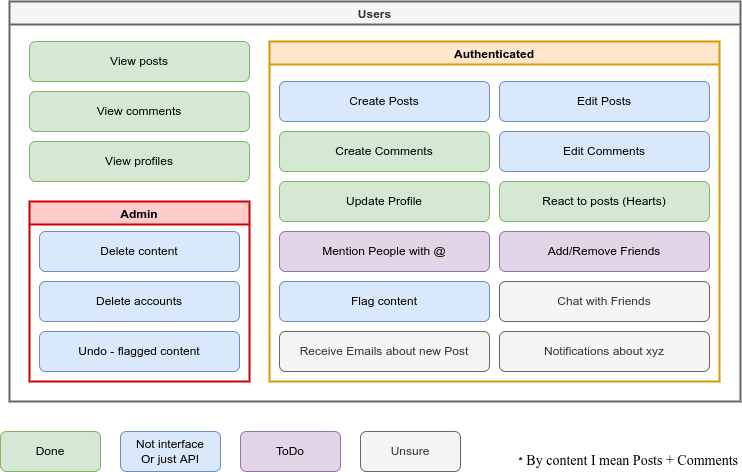
\includegraphics[height=0.5\textwidth]{../d_usecase.drawio}
        \caption{Use cases für alle Anwender. \href{https://github.com/MKrabs/Blog/blob/main/docs/d_usecase.drawio.png}{github link}}
        \label{fig:use-cases}
    \end{figure}


    \section{Technologies}\label{sec:technologies}

    \begin{itemize}
        \item Geplant ist Django mit SQLite3 (fullstack) zu nutzten.
        \item M\"oglicherweise wird der Service auf Django + Vue umgezogen, um eine asynchrone Single-page Application als Frontend zu haben.
    \end{itemize}
\end{document}
